\documentclass[12pt,a4paper]{ctexart}
\usepackage{geometry}
\usepackage{booktabs}
\usepackage{graphicx}
\usepackage{float}
\usepackage{amsmath}
\usepackage{longtable}
\geometry{margin=2.5cm}

\title{基于“公司名称+岗位名称”联合映射的\\20门类行业异质性分析报告}
\author{}
\date{2026-02-09}

\begin{document}
\maketitle

\section{研究目标与数据口径}
本报告基于已完成的“公司名称+岗位名称联合映射到20个经济活动门类（A--T）”结果，分析行业异质性在两条维度上的差异：
\begin{itemize}
    \item \textbf{维度一：岗位综合化程度}（Global LDA 指标：Entropy/HHI）；
    \item \textbf{维度二：技能结构演化}（Alignment 指标：技能存活率/重组率）。
\end{itemize}

核心输入与结果底表如下：
\begin{itemize}
    \item 岗位级主表：\texttt{data/Heterogeneity/master\_joint\_industry20\_analysis.csv}
    \item 年度综合化表：\texttt{data/Heterogeneity/yearly\_industry20\_entropy\_metrics.csv}
    \item 窗口存活率表：\texttt{data/Heterogeneity/industry20\_alignment\_survival\_metrics.csv}
\end{itemize}

联合映射规则采用多源打分：公司行业先验、公司初级分类先验、公司名称关键词、岗位名称关键词；最终输出 \texttt{industry20\_code}、\texttt{mapping\_confidence} 与 \texttt{mapping\_source}。

\section{数据质量核验}
\subsection{总体质量}
\begin{table}[H]
\centering
\caption{联合映射质量摘要}
\begin{tabular}{ll}
\toprule
指标 & 数值 \\
\midrule
主表样本量 & 7,768,501 \\
年份覆盖 & 2016--2025 \\
\texttt{U 未识别/其他} 占比 & 17.78\% \\
映射置信度均值 & 0.730 \\
映射置信度中位数 & 0.914 \\
\bottomrule
\end{tabular}
\end{table}

\subsection{20个经济活动门类口径（A--T）}
\begin{longtable}{ll}
\caption{行业异质性分析采用的20门类定义} \\
\toprule
代码 & 门类 \\
\midrule
\endfirsthead
\toprule
代码 & 门类 \\
\midrule
\endhead
\bottomrule
\endfoot
A & 农、林、牧、渔业 \\
B & 采矿业 \\
C & 制造业 \\
D & 电力、热力、燃气及水生产和供应业 \\
E & 建筑业 \\
F & 批发和零售业 \\
G & 交通运输、仓储和邮政业 \\
H & 住宿和餐饮业 \\
I & 信息传输、软件和信息技术服务业 \\
J & 金融业 \\
K & 房地产业 \\
L & 租赁和商务服务业 \\
M & 科学研究和技术服务业 \\
N & 水利、环境和公共设施管理业 \\
O & 居民服务、修理和其他服务业 \\
P & 教育 \\
Q & 卫生和社会工作 \\
R & 文化、体育和娱乐业 \\
S & 公共管理、社会保障和社会组织 \\
T & 国际组织 \\
\end{longtable}

\subsection{年度可用性约束}
在按年$\times$行业统计中，采用 $sample\_n \geq 50$ 作为有效单元阈值。该阈值下，2019 年有效行业数仍为 0，2020 年恢复到 8 个，2025 年为 18 个；但 2025 年总样本量仅 12,209，故该年行业均值仍需谨慎解释。

\section{结果一：岗位综合化的行业异质性（Entropy）}
\subsection{年度趋势}
\begin{figure}[H]
    \centering
    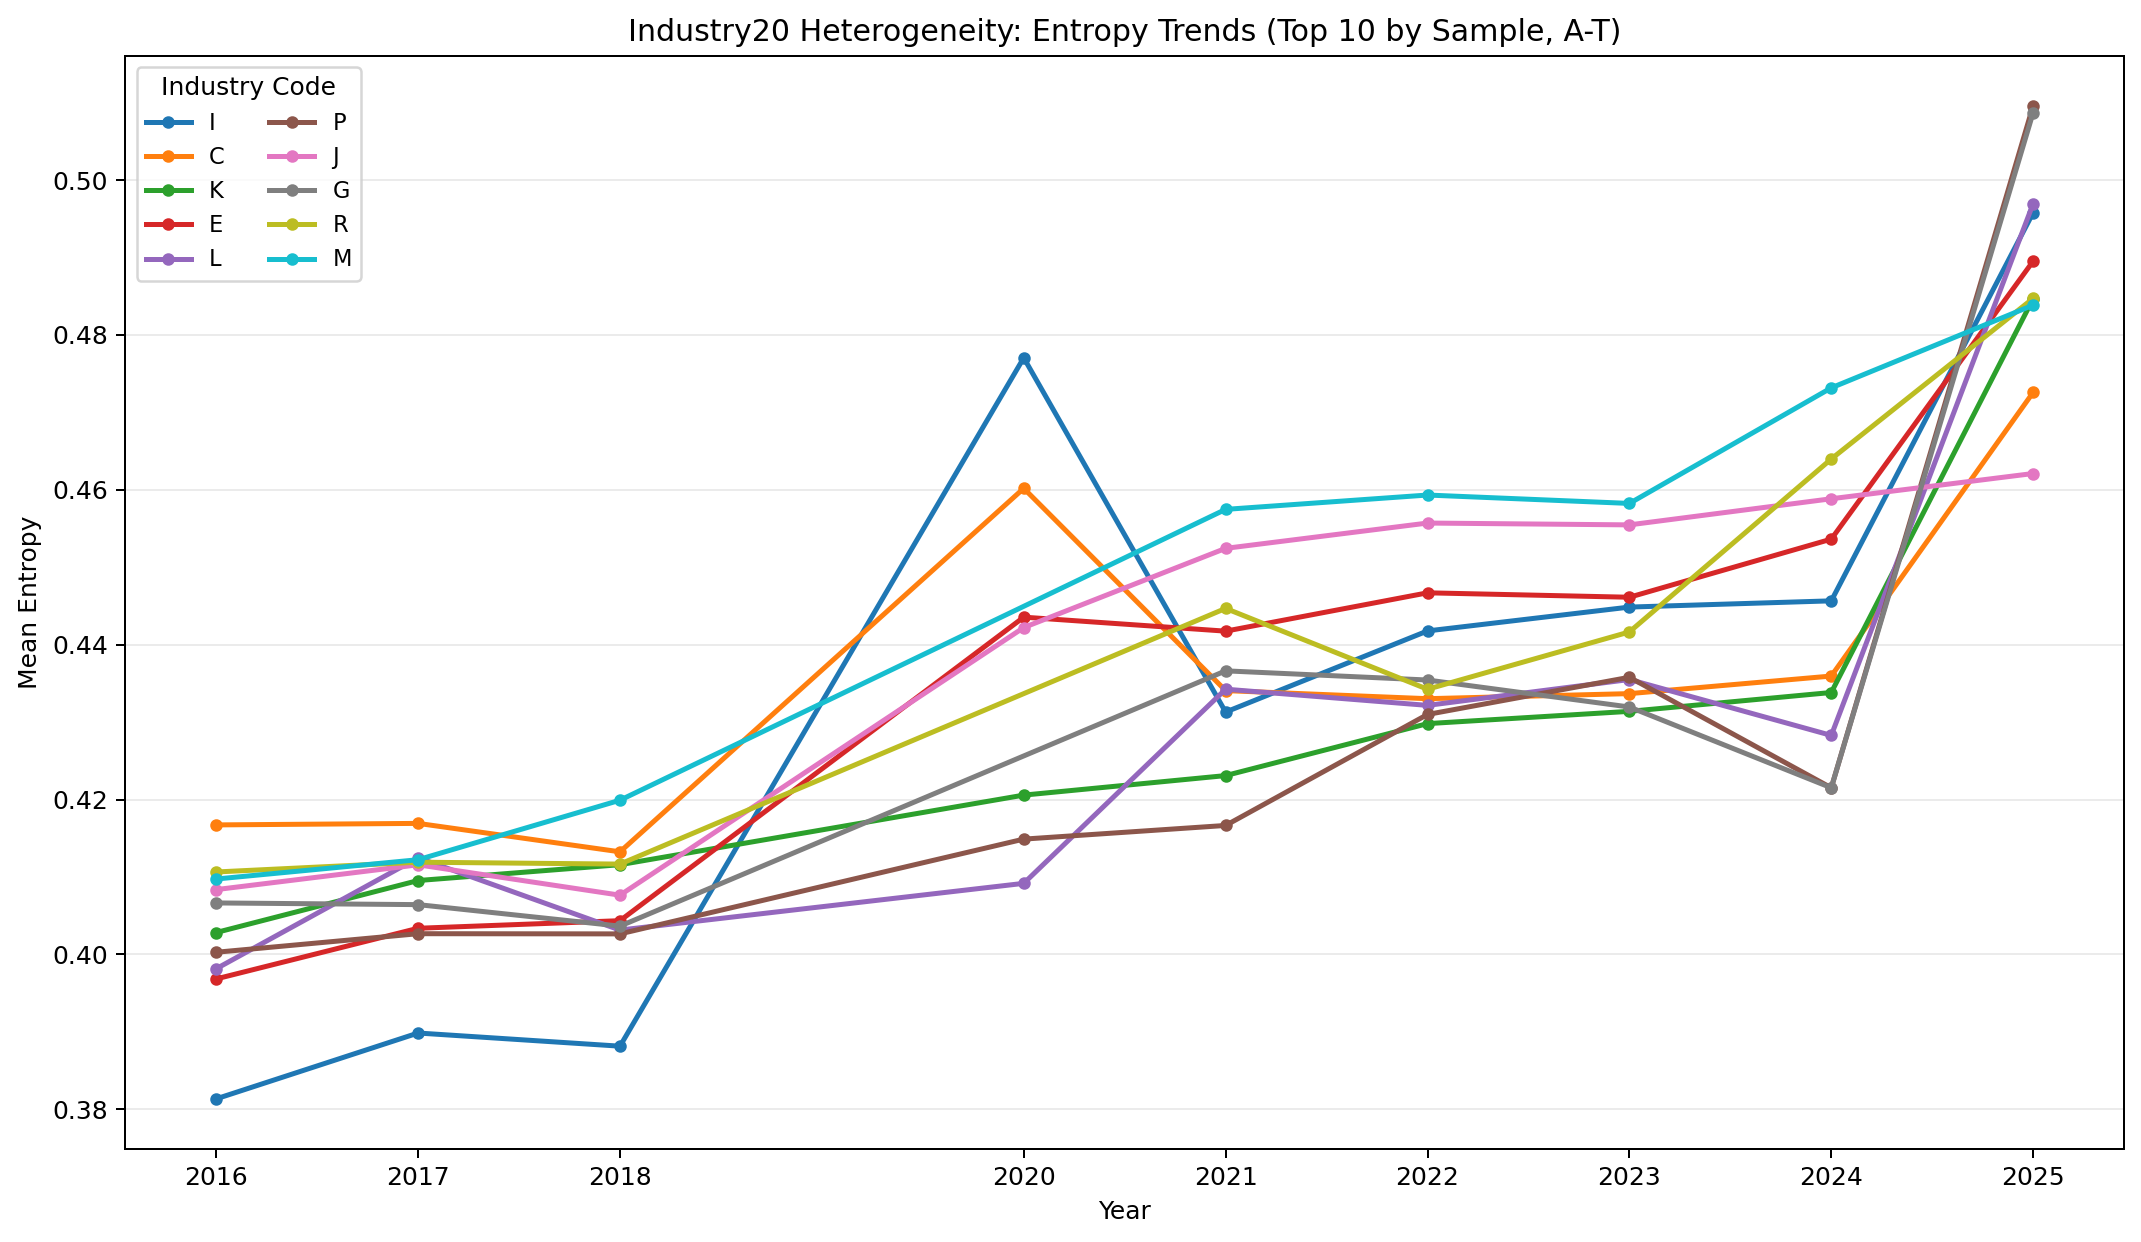
\includegraphics[width=0.95\textwidth]{figures/industry20_entropy_trend_top10.png}
    \caption{20门类行业异质性：Entropy 年度趋势（A--T，按总样本量前10行业）}
\end{figure}

图中可见，多数头部行业在 2016--2024 期间呈现 Entropy 上行，即岗位技能组合趋于更综合化。尽管在阈值放宽后 2025 年达阈值行业数明显增加，但由于其总样本量仍显著偏小，跨期叙事依然应以 2016--2018 与 2021--2024 的对比为主，2025 年作为补充观察。

\subsection{“追赶型”行业识别（2016 基线 vs 2025 增长）}
\begin{figure}[H]
    \centering
    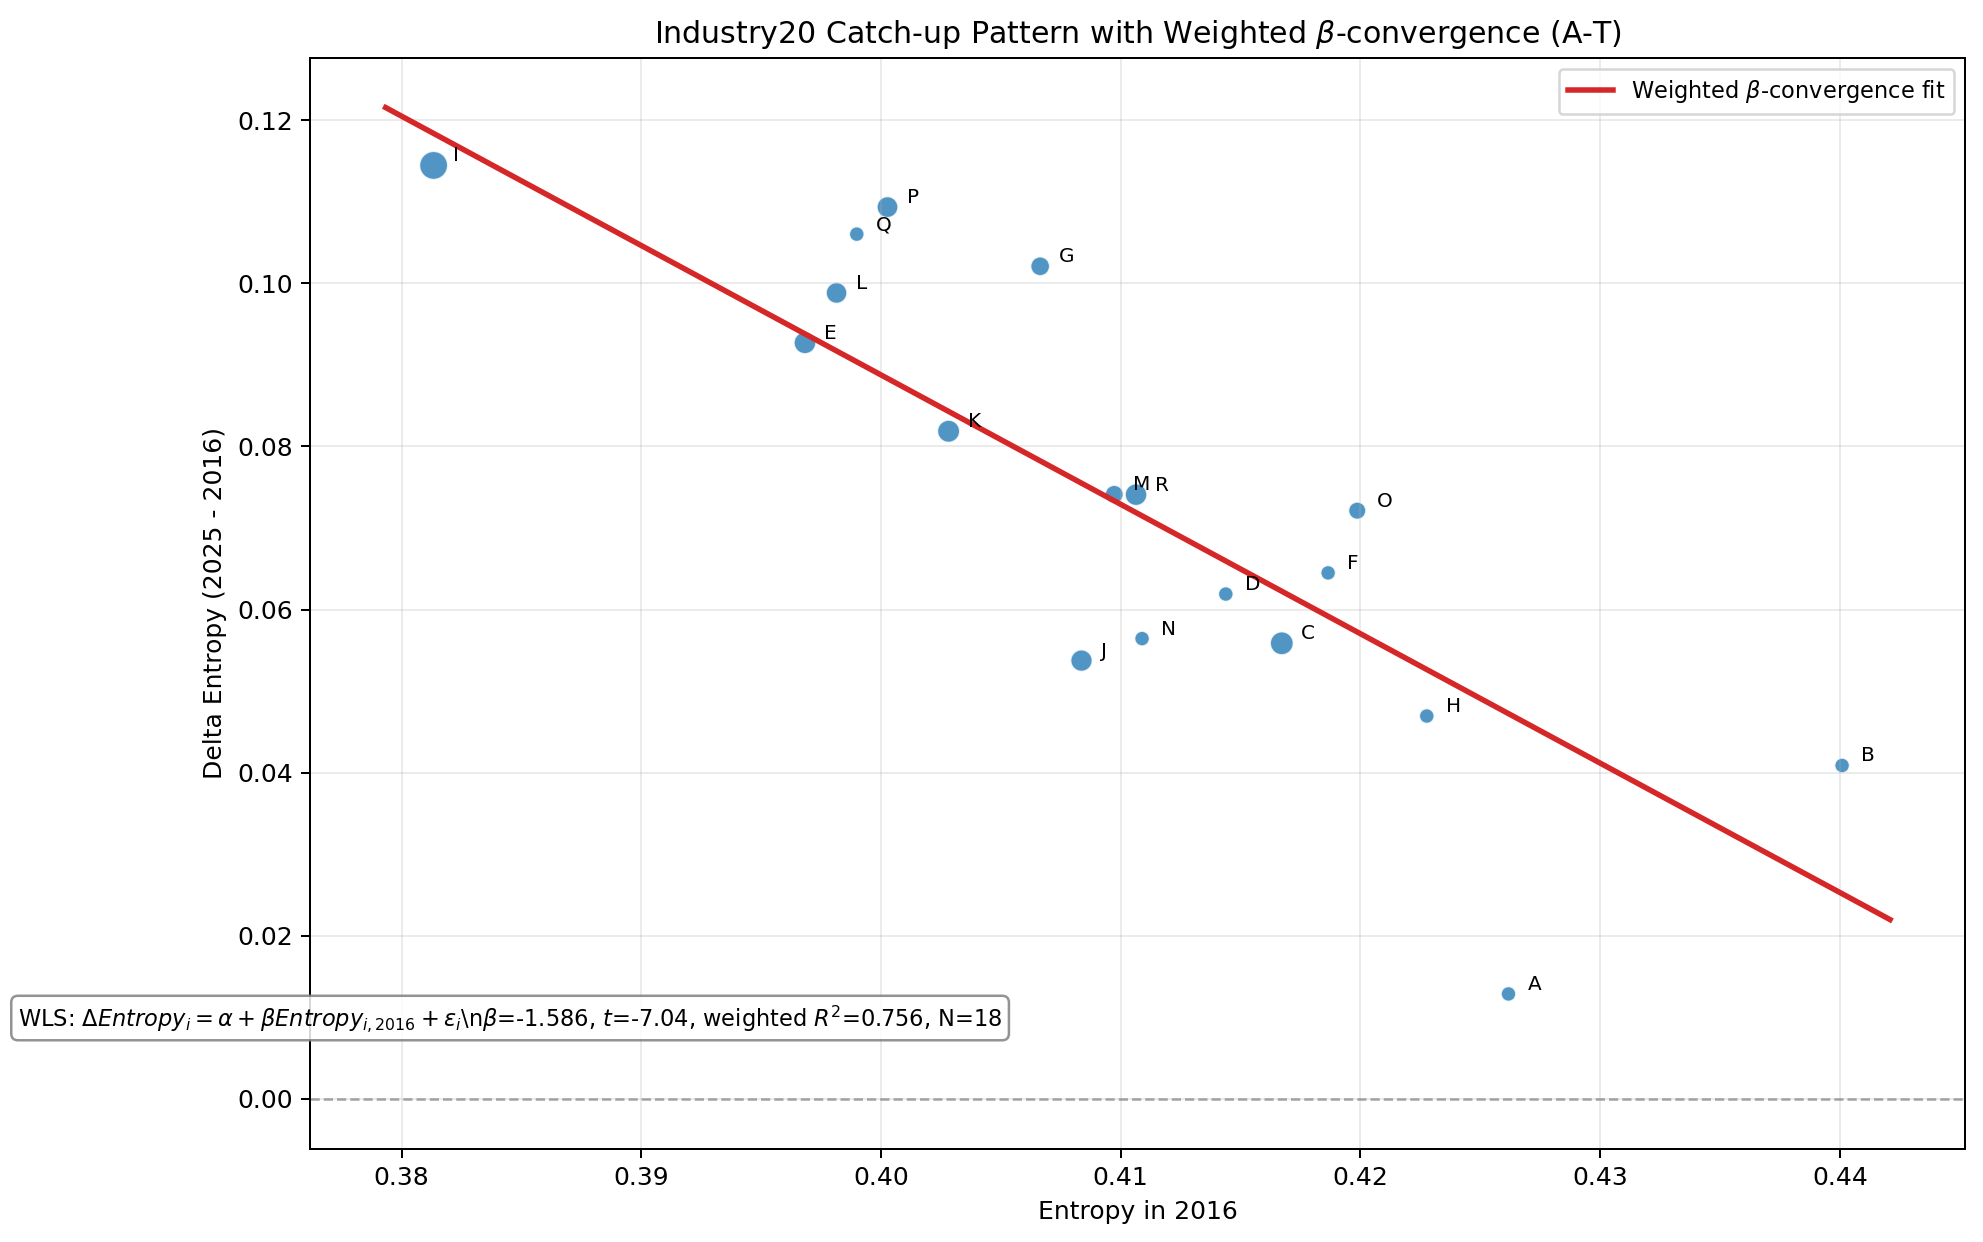
\includegraphics[width=0.92\textwidth]{figures/industry20_entropy_growth_scatter_2016_2025.png}
    \caption{行业追赶特征主图：2016 年初始 Entropy 与 2016$\rightarrow$2025 增量（含加权 $\beta$-convergence 回归线）}
\end{figure}

在保留散点主图的基础上，3.2 同时引入 $\beta$-convergence 识别：
\[
\Delta Entropy_i=\alpha+\beta \cdot Entropy_{i,2016}+\varepsilon_i
\]
其中 $\Delta Entropy_i=Entropy_{i,2025}-Entropy_{i,2016}$，并以行业平均样本量（\texttt{sample\_avg}）作为权重进行加权最小二乘估计。估计结果为 $\hat{\beta}=-1.586$（$t=-7.04$，加权 $R^2=0.756$，$N=18$），表明初始 Entropy 越低的行业，后续提升幅度越大，存在显著“追赶效应”。
回归系数已保存于 \texttt{data/Heterogeneity/industry20\_beta\_convergence\_wls.csv}。

基于有效行业（2016 与 2025 均达阈值）计算，Entropy 增幅较高的行业包括：
\begin{itemize}
    \item I 信息传输、软件和信息技术服务业：$\Delta Entropy = +0.114$（+30.01\%）；
    \item P 教育：$+0.109$（+27.32\%）；
    \item Q 卫生和社会工作：$+0.106$（+26.57\%）；
    \item G 交通运输、仓储和邮政业：$+0.102$（+25.10\%）；
    \item L 租赁和商务服务业：$+0.099$（+24.82\%）。
\end{itemize}
需注意，教育与卫生在 2025 年样本量较小（分别为 88 与 179），其高增幅应结合样本规模谨慎解读。这表明行业间不仅存在静态差距，也存在明显的“动态追赶”差异。

\section{结果二：技能结构演化的行业异质性（Alignment 存活率）}
定义行业技能存活率为：
\[
SurvivalRate_{i,t\rightarrow t+1}=\frac{n_{\text{survive},i,t\rightarrow t+1}}{n_{\text{source},i,t}}
\]
并以 $ReorganizationRate=1-SurvivalRate$ 表示结构重组强度。

\subsection{窗口热力图（头部行业）}
\begin{figure}[H]
    \centering
    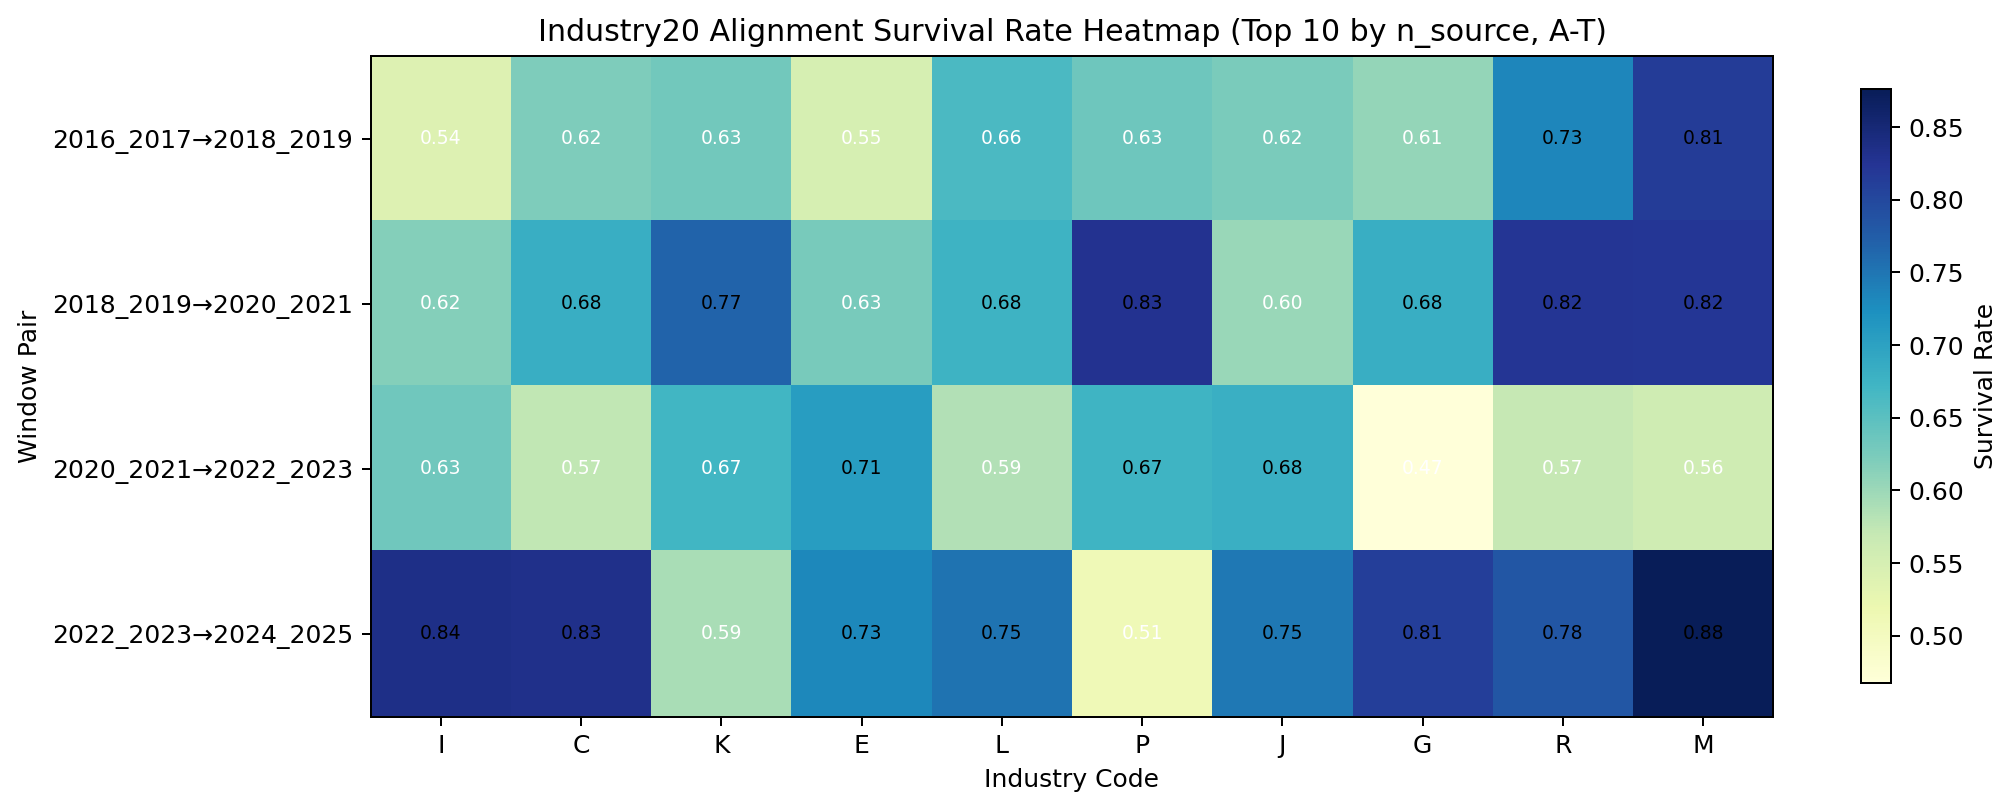
\includegraphics[width=0.98\textwidth]{figures/industry20_alignment_survival_heatmap_top10.png}
    \caption{20门类行业异质性：Alignment 技能存活率热力图（A--T，按 $n\_{\text{source}}$ 前10行业）}
\end{figure}

\subsection{行业排序结果}
按四个窗口平均后，存活率较高的行业为：
\begin{itemize}
    \item T 国际组织（0.930，样本量很小）；
    \item M 科学研究和技术服务业（0.768）；
    \item R 文化、体育和娱乐业（0.727）；
    \item N 水利、环境和公共设施管理业（0.681）；
    \item C 制造业（0.677）。
\end{itemize}

存活率较低的行业为：
\begin{itemize}
    \item Q 卫生和社会工作（0.595）；
    \item F 批发和零售业（0.611）；
    \item S 公共管理、社会保障和社会组织（0.627，样本量较小）；
    \item G 交通运输、仓储和邮政业（0.642）；
    \item O 居民服务、修理和其他服务业（0.642）。
\end{itemize}

\subsection{窗口总体变化（加权口径）}
按行业窗口样本量 $n\_{\text{source}}$ 加权后，总体存活率为：
\begin{itemize}
    \item 2016--2017 $\rightarrow$ 2018--2019：0.617（重组率 0.383）；
    \item 2018--2019 $\rightarrow$ 2020--2021：0.684（重组率 0.316）；
    \item 2020--2021 $\rightarrow$ 2022--2023：0.615（重组率 0.385）；
    \item 2022--2023 $\rightarrow$ 2024--2025：0.750（重组率 0.250）。
\end{itemize}
该结果表明结构重组并非单调演进，而是存在阶段性波动。

\section{结论与下一步}
\subsection{主要结论}
\begin{itemize}
    \item 在 20 门类口径下，岗位综合化（Entropy）存在稳定行业差异，且多数头部行业在 2016--2024 呈上行趋势；
    \item 不同行业技能结构稳定性（Alignment 存活率）差异显著，部分行业长期更稳定，部分行业长期更易重组；
    \item “综合化增速高”与“结构存活率高”并不等价，提示两类指标应联合解释。
\end{itemize}

\subsection{方法边界}
\begin{itemize}
    \item 即便阈值放宽到 $sample\_n \geq 50$，2019 年仍几乎不可用，2025 年虽覆盖行业较全但总样本量偏低，跨期可比性仍受限制；
    \item \texttt{U 未识别/其他} 仍占 17.78\%，需要持续优化映射规则；
    \item 后续正式实证建议以 2016--2018 与 2021--2024 为主区间，并进行稳健性检验（阈值敏感性、加权/非加权对照）。
\end{itemize}

\end{document}
